\chapter{Development process}
\todo{intro schrijven}

\section{Diffusion model used: FLUX.1 [dev]} \label{sec:Models used}
The diffusion model used in this thesis is called FLUX.1 (\cite{black_forest_labs_announcing_2024}), a text-to-image diffusion model released on August 1, 2024, in three variants: FLUX.1 [pro], [dev], and [schnell]. Of these three variants, only [dev] and [schnell] have open-source weights and thus support local use and fine-tuning via low-rank adaptation (LoRA).\\
Following preliminary experimentation, only FLUX.1 [dev] is used in this thesis, because of its superior integration with Ostris' FLUX.1 [dev] LoRA trainer. LoRAs trained with the [dev] trainer also function with FLUX.1 [schnell], but yield lower-quality output images. Training LoRAs specifically for FLUX.1 [schnell] is also possible, although one would need to use an adapter for that (the adapter can be found on \url{https://huggingface.co/ostris/FLUX.1-schnell-training-adapter}{https://huggingface.co/ostris/FLUX.1-schnell-training-adapter}). This option was not tested.
\section{Image generation techniques}
\subsection{Text-to-Image}
\todo{kleine intro bij schrijven}
\subsubsection{ChatGPT} \label{sec:ChatGPT}
To streamline the prompt engineering process, the researcher trained a custom GPT named 'LoRA prompt generator' (\href{https://chatgpt.com/g/g-68279d68896c81918191491b79281abe-lora-prompt-generator}{link}) to output high-quality prompts consisting of a six-part structure. A GPT is a custom version of ChatGPT that can follow specific instructions (\cite{openai_introducing_2023}). This option was chosen because of the combination of accessibility (since GPTs are easy to configure without knowing a lot about large language models) and effectivity.\\
The recommended models to use for this GPT are GPT-o3 and GPT-o4-mini \footnote{Since the release of GPT-5 on august 7, 2025, these models are not directly accessible anymore. It is therefore recommended to use GPT-5 Thinking.}, because they are able to directly integrate images into their chain of thought (\cite{openai_introducing_2025}, section 'Thinking with images').\\
The researcher can write a prompt in natural language, and the GPT reformulates it into a six-part prompt following a fixed structure. This structure facilitates easier analysis of the prompts. Table \ref{tab:gptprompt} dissects a representative output generated by the GPT to illustrate the structure. \\

\begin{table}[H]
  \centering
  \begin{tabular}{l p{0.6\textwidth}}
    \toprule
    Structure & Prompt segment \\
    \midrule
    1. Trigger word 
    & Stampbeton \\
    2. Subject
    & shapes the rugged elegance of a countryside farmhouse, where the front facade stands defined by sturdy stamped concrete walls that echo the texture of hand-laid stone. \\
    3. Attributes on the subject
    & A gently slanted roof clad in red shingles crowns the structure, lending a traditional warmth that contrasts the cool, tactile mass of the concrete below. On the front elevation, a single wooden door punctuates the left side, its weathered grain harmonizing with the rustic palette, while a solitary window on the right offers a glimpse into the home’s quiet interior, framed by thick concrete reveals. \\
    4. Surroundings
    & The house is nestled into a soft rural clearing, flanked by wild grasses and a gravel path that leads up to the entrance, with distant hedgerows and fencing marking the rhythm of nearby fields. \\
    5. Atmosphere 
    & Overhead, a wide expanse of blue sky peeks through the rolling coverage of dense, moody clouds, diffusing the daylight into a serene, shadowless glow. \\
    6. Style 
    & Rendered in photorealistic style, the scene captures the raw materiality and quiet strength of this rural retreat, balanced by a subtle, cinematic atmosphere. \\
    \bottomrule
  \end{tabular}
  \caption{The six-part structure used to generate every prompt in this thesis.\\}
  \label{tab:gptprompt}
\end{table}
Users can edit the output prompt to their preference, reducing the workload compared to writing a high-quality prompt from scratch. \\
Because every image generated in this thesis is a pair (with and without LoRA; see section \ref{sec:Workflow used to generate images}), the GPT was designed to output two prompts: one with the trigger words and one with their English equivalents that the base model FLUX.1 [dev] can interpret. This ensures the comparison is as fair as possible.

\begin{table}[H]
    \centering
    \begin{tabular}{ll}
        \toprule
         Stampbeton & Stamped concrete\\
         3Deffect & 3D effect\\
         Geleding & Division \\
         Modulariteit & Modularity\\
         Ghoek & Curvature\\
         Plintwerking & Plinth effect\\
         \bottomrule
    \end{tabular}
    \caption{All of the trigger words and their English counterpart.}
    \label{tab:triggerwords}
\end{table}

\subsection{Image-to-Image}
\subsubsection{ControlNet}
To generate images based on sketches or images of the architects, ControlNet (\cite{zhang_adding_2023}) was used, a technique to add compositional control to large diffusion models such as FLUX. The ControlNet model used in this thesis is the 'union pro' model by Shakker Labs (\url{https://huggingface.co/Shakker-Labs/FLUX.1-dev-ControlNet-Union-Pro/tree/main}), which includes several preprocessors.
\section{Interface used to generate images} \label{sec:Workflow used to generate images}
\subsection{ComfyUI}
\sloppy
The interface used to generate images in this thesis is called ComfyUI (\href{https://www.comfy.org/}{comfy.org}), an open source node-based user interface. Alternatives such as Automatic1111, Fooocus and InvokeAI were considered; however, ComfyUI was selected due to two primary advantages. 
\begin{enumerate}
    \item Reproducability: generated images embed the complete 'workflow' used to create it (see \href{https://docs.comfy.org/development/core-concepts/workflow}{docs.comfy.org} for further explanations). Since reproducability is an important aspect of research, this is a very attractive feature, as it allows researchers to retrace how every AI-generated image in this thesis was created.
    \item Customizability: by using fundamental building blocks ('nodes', see \href{https://docs.comfy.org/development/core-concepts/nodes}{docs.comfy.org}), ComfyUI users can create their own workflows to meet various needs, and can also write and implement custom nodes to further customize workflows.
\end{enumerate}
Figure \ref{fig:comfy interface} illustrates the default ComfyUI workflow, which can generate one image from a positive and a negative prompt.
\begin{figure}[H]
    \centering
    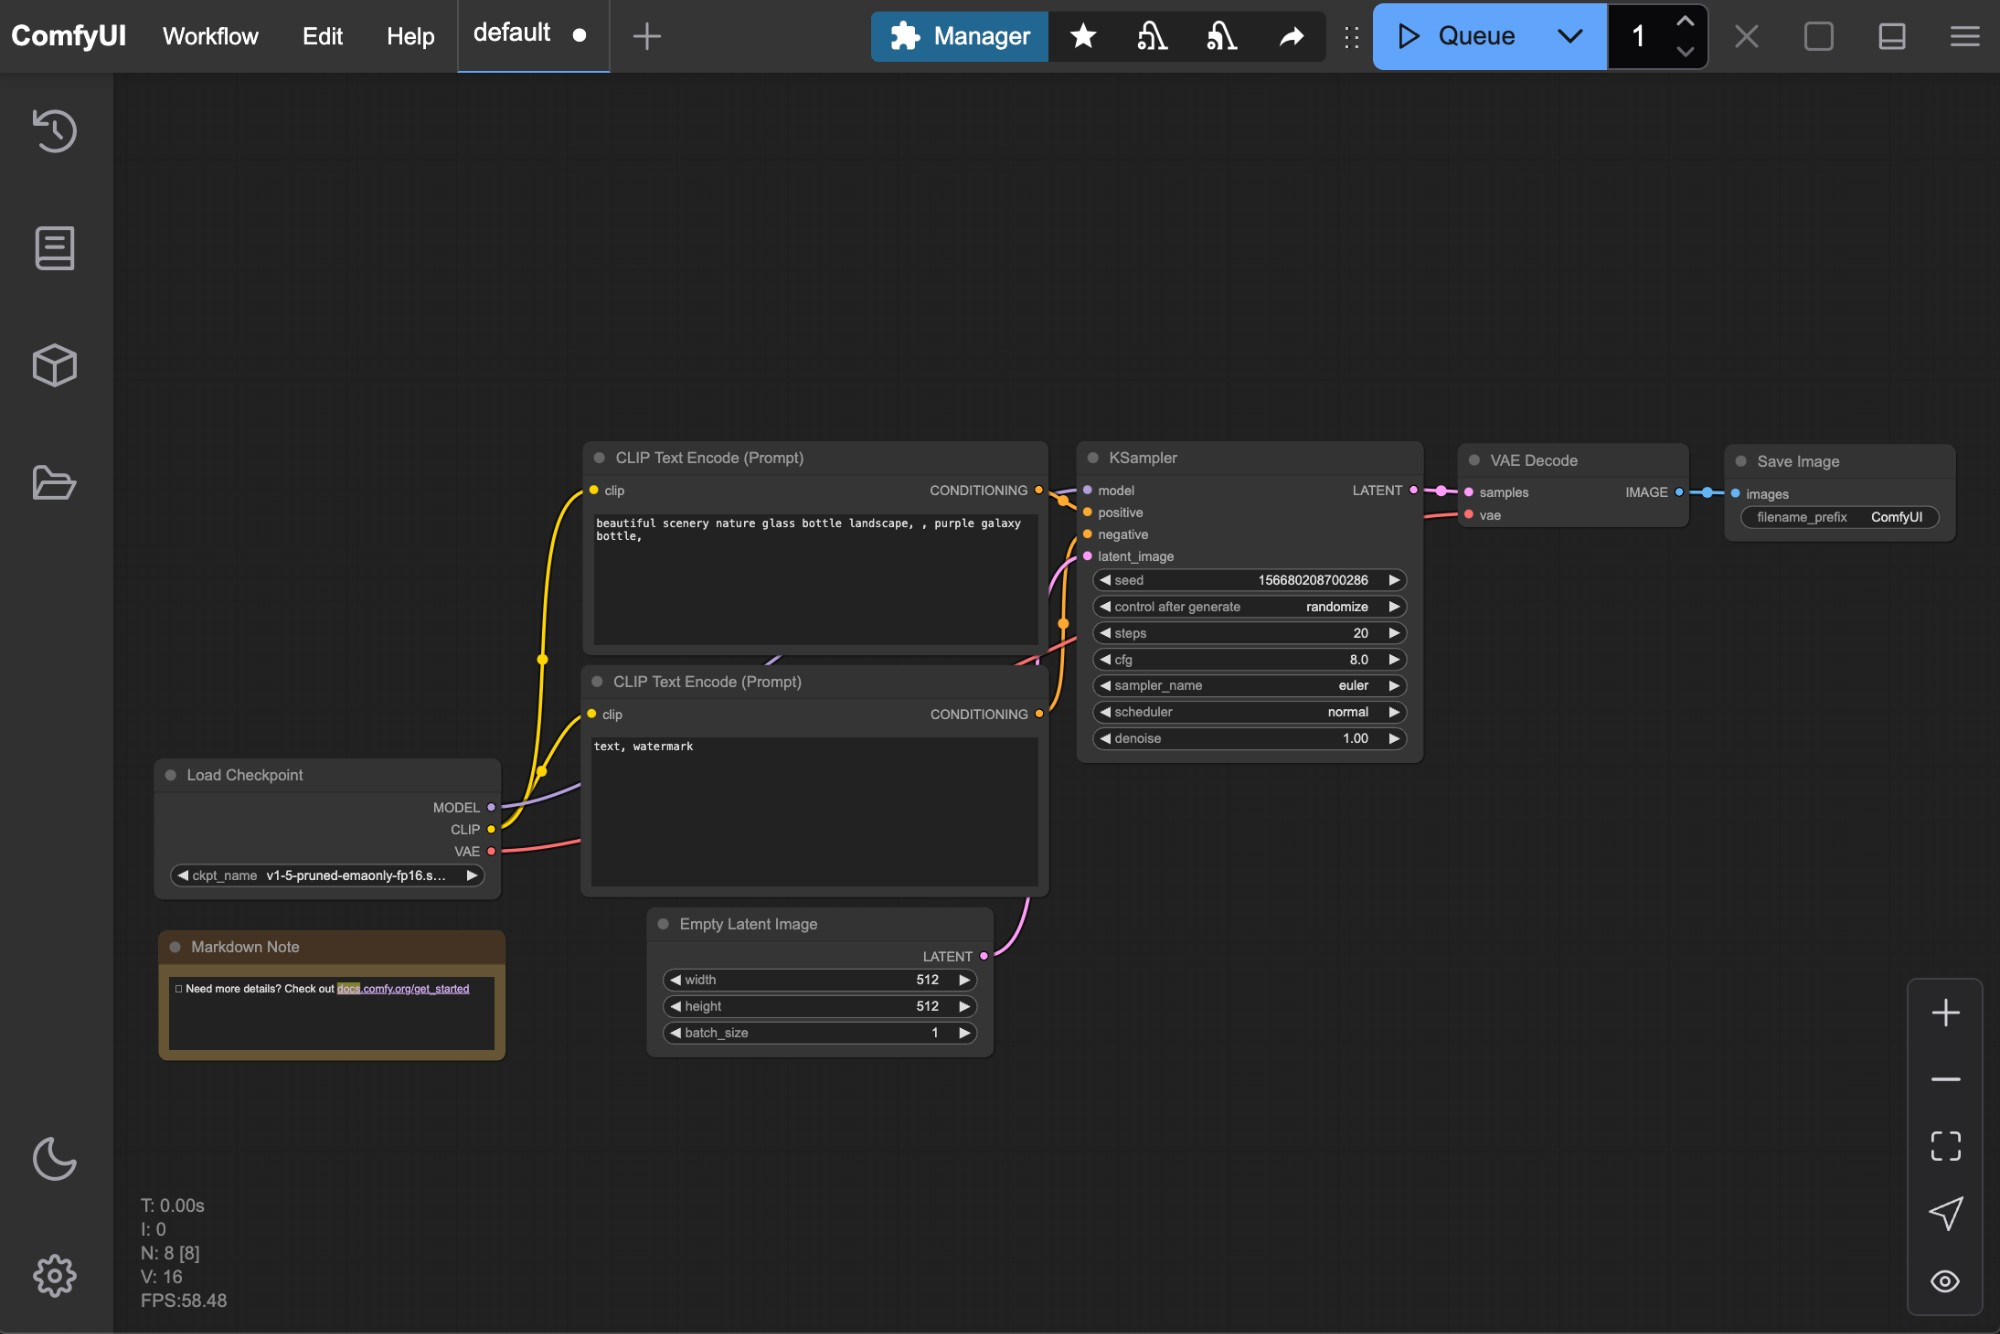
\includegraphics[width=0.8\linewidth]{Images//Methodology/comfyui_new_interface.jpg}
    \caption{The default workflow when starting ComfyUI.}
    \label{fig:comfy interface}
\end{figure}

To generate images, the researcher employed an online service called \textbf{ThinkDiffusion} (\href{https://www.thinkdiffusion.com/}{thinkdiffusion.com}) and rented a server with 48 gigabytes of video random-access memory (VRAM), which is capable of generating one image in about 30 seconds when using FLUX.1 [dev]. The version of ComfyUI used is ComfyUI v0.3.44, the latest available in July 2025.
\subsection{Workflow used in this thesis}
To generate all of the images in this thesis, the researcher employed a custom workflow developed by Swedish art director and youtuber Sebastian Kamph(\cite{sebastian_kamph_flux_2024}), which enables the use of ControlNets in combination with FLUX. To isolate and highlight the effect of LoRA on the generated output images, the workflow was modified into a new version (figure \ref{fig:own comfy workflow}) that generates two images per execution: one with LoRA enabled and one without. All other parameters, such as prompts and seed values, are held constant. Each time the workflow is executed, two images are simultaneously generated and displayed in the nodes on the bottom right of the workflow.\\ 
\begin{figure}[H]
    \centering
    \href{https://github.com/matijspeeters/Thesis/blob/main/Images/Methodology/workflow%20(5).png}{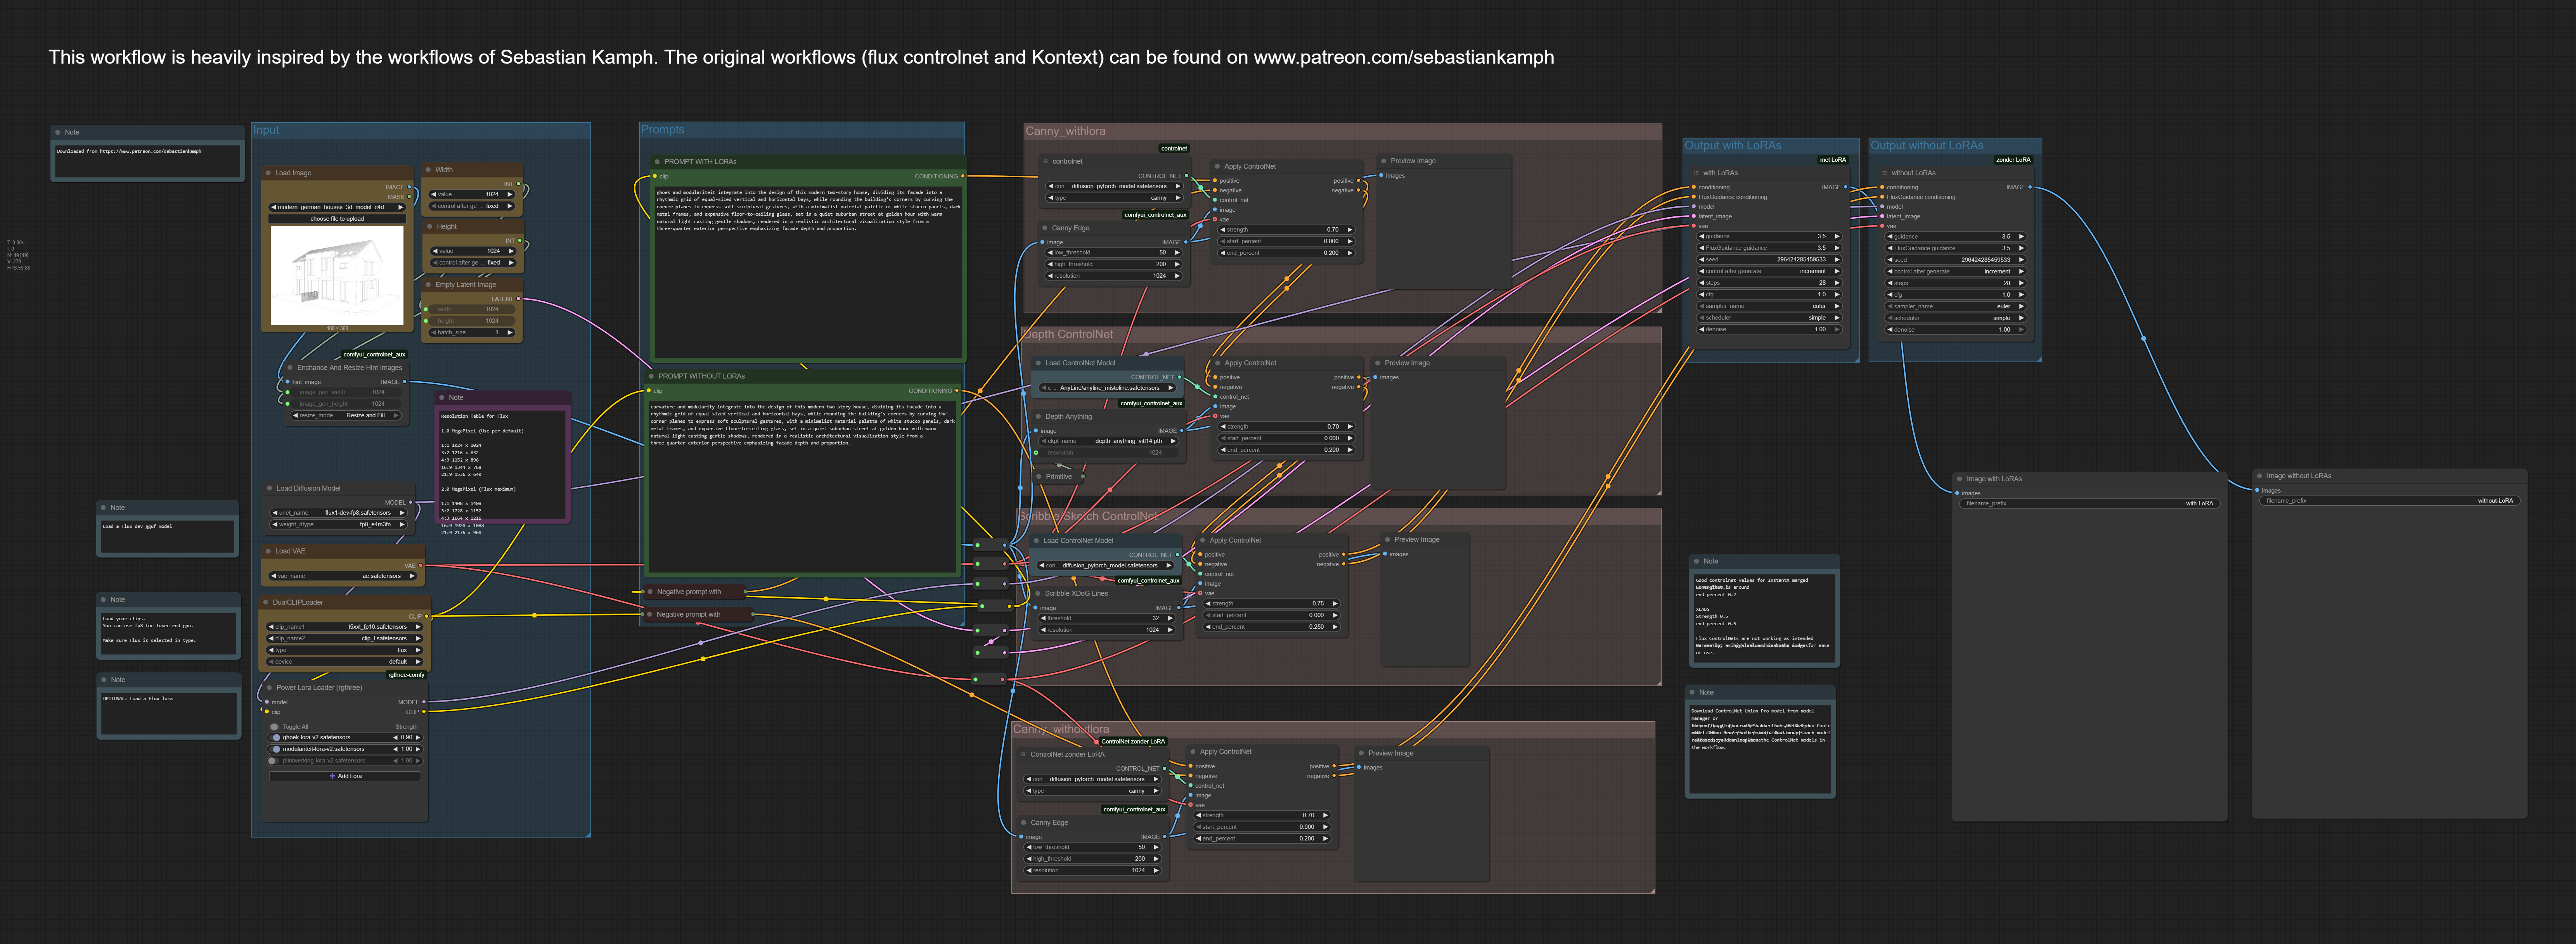
\includegraphics[width=\linewidth]{Images/Methodology/workflow (5).png}}
    \caption{The modified ComfyUI workflow, used to generate every image in this thesis.}
    \label{fig:own comfy workflow}
\end{figure}